\documentclass[11pt,fancy]{elegantbook}
\usepackage{float}

\title{Data Science Specialization}
\subtitle{Coursera Course}

\author{Shivani Nandani}
\institute{Johns Hopkins University}
\date{January 2022}
\version{1.0}
\bioinfo{Bio}{A ten-course introduction to data science.}

\extrainfo{Victory won\rq t come to us unless we go to it. }

\cover{cover.jpg}

\definecolor{customcolor}{RGB}{43, 56, 86}
\colorlet{coverlinecolor}{customcolor}


\begin{document}

\maketitle

\frontmatter
\tableofcontents

\mainmatter

\chapter{The Data Scientist\rq s Toolbox}
Course\cite{course1} outcomes:
\begin{itemize}
    \item an introduction to the main tools and ideas in the data scientist's toolbox
    \item an overview of the data, questions, and tools that data analysts and data scientists work with
    \item two components:
          \begin{enumerate}
              \item a conceptual introduction to the ideas behind turning data into actionable knowledge
              \item a practical introduction to the tools that will be used in the program like version control, markdown, git, GitHub, R, and RStudio
          \end{enumerate}
\end{itemize}

\section{What is data science?}
\begin{itemize}
    \item can mean different things to different people
    \item at it's core, data science is using data to answer questions
    \item involves
          \begin{itemize}
              \item statistics, computer science, mathematics
              \item data cleaning and formatting
              \item data visualization
          \end{itemize}
    \item An Economist Special Report sums up this melange of skills well - they state that a data scientist is broadly defined as someone "who combines the skills of software programmer, statistician and storyteller slash artist to extract the nuggets of gold hidden under mountains of data"
\end{itemize}

\section{What is big data?}
\begin{itemize}
    \item vast amount of data collected in currently
    \item rise of inexpensive computing
    \item \textbf{volume} - big data involves large datasets - and these large datasets are becoming more and more routine
    \item \textbf{velocity} - generated and collected faster than ever before
    \item \textbf{variety} - different types of data
\end{itemize}
\begin{figure}[H]
    \centering
    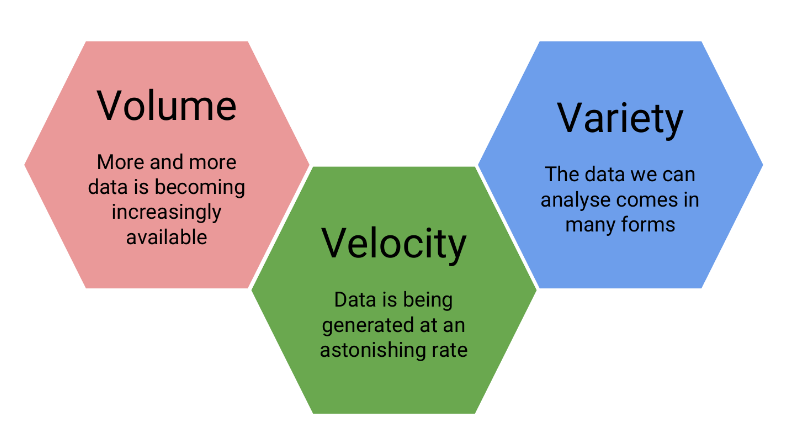
\includegraphics[width=7cm]{ch1_1.png}
    \caption{A summary of three qualities that characterize big data}
    \label{fig:big_data}
\end{figure}

\section{What is a data scientist?}
\begin{itemize}
    \item the most basic of definitions would be that a data scientist is somebody who uses data to answer questions
          \begin{figure}[H]
              \centering
              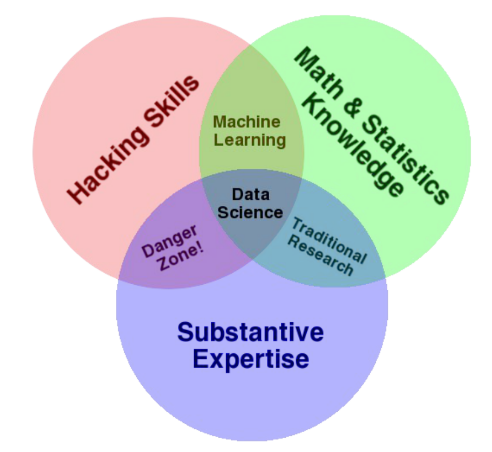
\includegraphics[width=5cm]{ch1_2.png}
              \caption{Drew Conway's Venn diagram of data science}
              \label{fig:data_scientist_dia}
          \end{figure}
    \item according to the illustrative Venn diagram\footnote{\url{http://drewconway.com/zia/2013/3/26/the-data-science-venn-diagram}}, data science is the intersection of three sectors - substantive expertise, hacking skills, and math and statistic
\end{itemize}

\section{What is data science?}
\begin{itemize}
    \item Cambridge English Dictionary definition - \textit{Information, especially facts or numbers, collected to be examined and considered and used to help decision-making.}
    \item Wikipedia definition - \textit{A set of values of qualitative or quantitative variables.}
    \item both these definitions say that data is values of numbers or facts but the Cambridge definition focuses more on the \textit{what} it is used for while the wikipedia definition talks about what data entails. here, "a set of values" talks about the population, the set of a whole that you are trying to discover something about. The "variables" are measurements or characteristics of an item (example - height of a person). It can be either qualitative or quantitative.
    \item common types of messy data:
          \begin{itemize}
              \item sequencing data
              \item population census data
              \item electronic media records (EMR) and other large datasets
              \item geographic information system (GIS) data (mapping)
              \item image analysis and image extrapolation
              \item language and translations
              \item website traffic
              \item personal/ad data (e.g.: facebook, netflix predictions etc.)
          \end{itemize}
    \item Sample project - \href{https://hilaryparker.com/2013/01/30/hilary-the-most-poisoned-baby-name-in-us-history/}{Hilary: the most poisoned baby name in US history}
\end{itemize}

\section{R programming language}
\begin{itemize}
    \item download from \href{https://cran.r-project.org/}{Comprehensive R Archive Network (CRAN)}
    \item focused on statistical analysis and graphics
    \item A package is not to be confused with a library (these two terms are often conflated in colloquial speech about R). A library is the place where the package is located on your computer. To think of an analogy, a library is, well, a library… and a package is a book within the library. The library is where the books/packages are located.
\end{itemize}

\section{Types of Data Science}
There are, broadly speaking, six categories in which data analyses fall.
\begin{enumerate}
    \item Descriptive
    \item Exploratory
    \item Inferential
    \item Predictive
    \item Causal
    \item Mechanistic
\end{enumerate}

\subsection{Descriptive analysis}
The goal of descriptive analysis is to describe or summarize a set of data. Whenever you get a new dataset to examine, this is usually the first kind of analysis you will perform. Descriptive analysis will generate simple summaries about the samples and their measurements.
\par This type of analysis is aimed at summarizing your sample - not for generalizing the results of the analysis to a larger population or trying to make conclusions. Description of data is separated from making interpretations; generalizations and interpretations require additional statistical steps.
\par Some examples of purely descriptive analysis can be seen in censuses. Here, the government collects a series of measurements on all of the country's citizens, which can then be summarized. Here, you are being shown the age distribution in the US, stratified by sex. The goal of this is just to describe the distribution. There is no inferences about what this means or predictions on how the data might trend in the future. It is just to show you a summary of the data collected.
\begin{figure}[H]
    \centering
    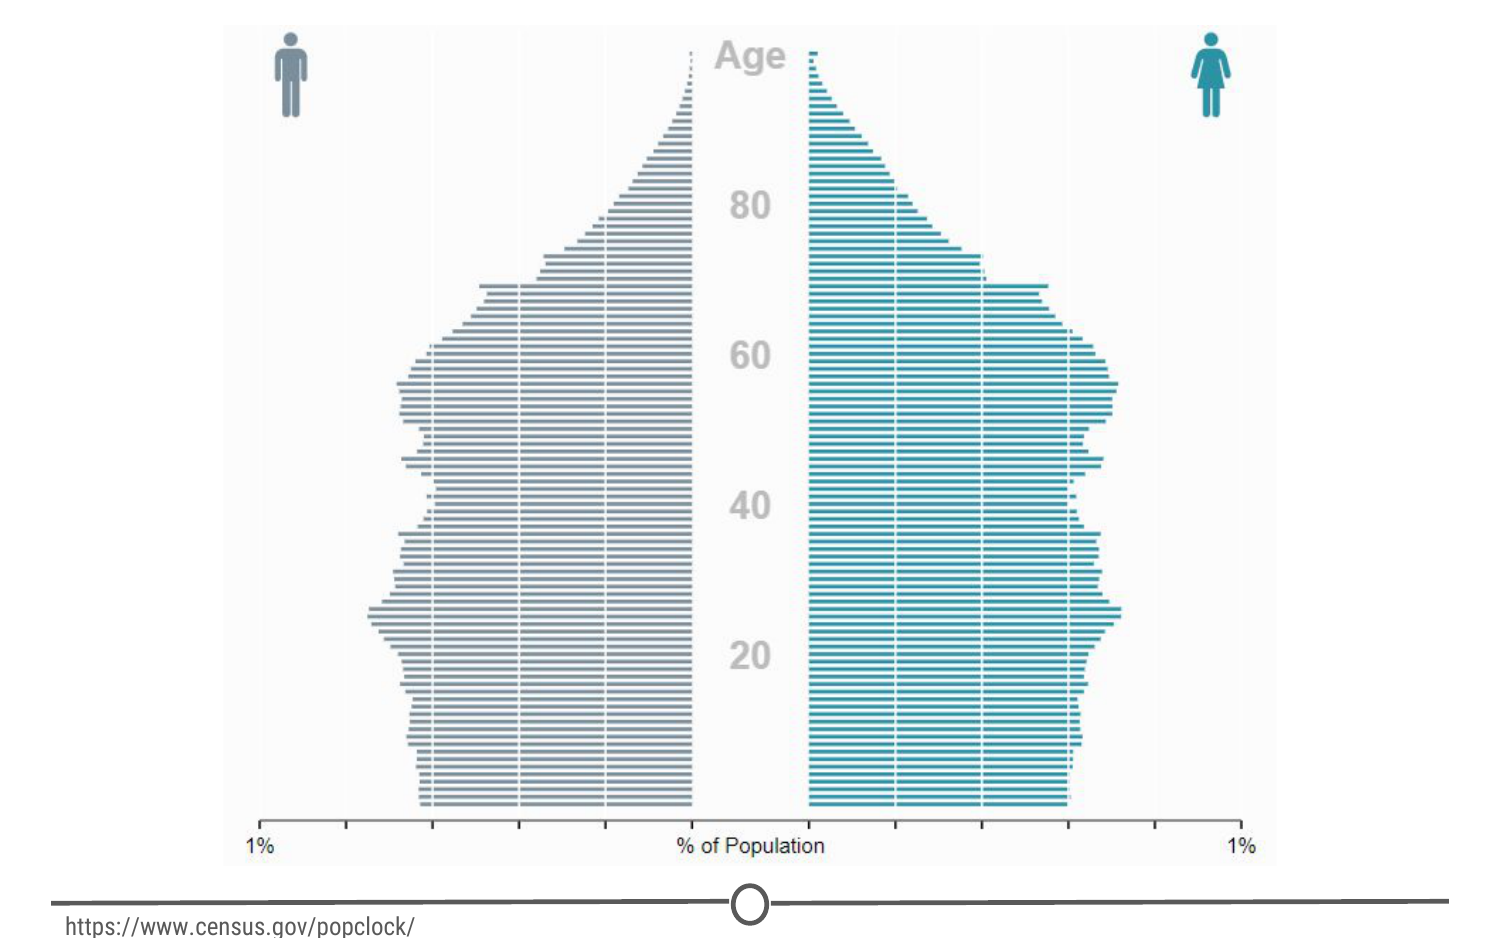
\includegraphics[width=12.5cm]{us_pop_data.png}
    \caption{A population pyramid describing the population distribution in the US}
    \label{fig:us_pop_data}
\end{figure}

\subsection{Exploratory analysis}
The goal of exploratory analysis is to examine or explore the data and find relationships that weren't previously known. Exploratory analyses explore how different measures might be related to each other but do not confirm that relationship as causative. "Correlation does not imply causation" - just because you observe a relationship between two variables during exploratory analysis, it does not mean that one necessarily causes the other.
\par Because of this, exploratory analysis, while useful for discovering new connections, should not be the final say in answering a question. It can allow you to formulate hypotheses and drive the design of future studies and data collection, but exploratory analysis alone should never be used as the final say on why or how data might be related to each other.

\subsection{Inferential analysis}
The goal of inferential analyses is to use a relatively small sample of data to infer or say something about the population at large. Inferential analysis is commonly the goal of statistical modelling, where you have a small amount of information to extrapolate and generalize that information to a larger group.
\par Inferential analysis typically involves using the data you have to estimate that value in the population and then give a measure of your uncertainty about your estimate. Since you are moving from a small amount of data and trying to generalize to a larger population, your ability to accurately infer information about the larger population depends heavily on your sampling scheme - if the data you collect is not from a representative sample of the population, the generalizations you infer won't be accurate for the population.
\par An example of inferential analysis is a study in which a subset of the US population was assayed for their life expectancy given the level of air pollution they experienced. This study uses the data they collected from a sample of the US population to infer how air pollution might be impacting life expectancy in the entire US.

\subsection{Predictive analysis}
The goal of predictive analysis is to use current data to make predictions about future data. Essentially, you are using current and historical data to find patterns and predict the likelihood of future outcomes.
\par Like in inferential analysis, your accuracy in predictions is dependent on measuring the right variables. If you aren't measuring the right variables to predict an outcome, your predictions aren't going to be accurate. Additionally, there are many ways to build up prediction models with some being better or worse for specific cases, but in general, having more data and a simple model generally performs well at predicting future outcomes.
\par All this being said, much like in exploratory analysis, just because one variable may predict another, it does not mean that one causes the other; you are just capitalizing on this observed relationship to predict the second variable.
\par A common saying is that prediction is hard, especially about the future. There aren't easy ways to gauge how well you are going to predict an event until that event has come to pass; so evaluating different approaches or models is a challenge.
\par We spend a lot of time trying to predict things - the upcoming weather, the outcomes of sports events, and in the example we'll explore here, the outcomes of elections. Nate Silver of FiveThirtyEight tries and predicts the outcomes of U.S. elections (and sports matches) using historical polling data and trends and current polling. FiveThirtyEight's models accurately predicted the 2008 and 2012 elections and was widely considered an outlier in the 2016 US elections, as it was one of the few models to suggest Donald Trump at having a chance of winning.

\subsection{Causal analysis}
The caveat to a lot of the analyses we've looked at so far is that we can only see correlations and can't get at the cause of the relationships we observe. Causal analysis fills that gap; the goal of causal analysis is to see what happens to one variable when we manipulate another variable - looking at the cause and effect of a relationship.
\par Generally, causal analyses are fairly complicated to do with observed data alone; there will always be questions as to whether it is correlation driving your conclusions or that the assumptions underlying your analysis are valid. More often, causal analyses are applied to the results of randomized studies that were designed to identify causation. Causal analysis is often considered the gold standard in data analysis, and is seen frequently in scientific studies where scientists are trying to identify the cause of a phenomenon, but often getting appropriate data for doing a causal analysis is a challenge.
\par One thing to note about causal analysis is that the data is usually analysed in aggregate and observed relationships are usually average effects; so, while on average giving a certain population a drug may alleviate the symptoms of a disease, this causal relationship may not hold true for every single affected individual.
\par As we've said, many scientific studies allow for causal analyses. Randomized control trials for drugs are a prime example of this. For example, one randomized control trial examined the effects of a new drug on treating infants with spinal muscular atrophy. Comparing a sample of infants receiving the drug versus a sample receiving a mock control, they measure various clinical outcomes in the babies and look at how the drug affects the outcomes.

\subsection{Mechanistic analysis}
Mechanistic analyses are not nearly as commonly used as the previous analyses - the goal of mechanistic analysis is to understand the exact changes in variables that lead to exact changes in other variables. These analyses are exceedingly hard to use to infer much, except in simple situations or in those that are nicely modeled by deterministic equations. Given this description, it might be clear to see how mechanistic analyses are most commonly applied to physical or engineering sciences; biological sciences, for example, are far too noisy of data sets to use mechanistic analysis. Often, when these analyses are applied, the only noise in the data is measurement error, which can be accounted for.
\par You can generally find examples of mechanistic analysis in material science experiments. Here, we have a study on biocomposites (essentially, making biodegradable plastics) that was examining how biocarbon particle size, functional polymer type and concentration affected mechanical properties of the resulting “plastic.” They are able to do mechanistic analyses through a careful balance of controlling and manipulating variables with very accurate measures of both those variables and the desired outcome.

\section{Experimental Design}
\begin{itemize}
    \item Experimental design is organizing an experiment so that you have the correct data (and enough of it!) to clearly and effectively answer your data science question. This process involves clearly formulating your question in advance of any data collection, designing the best set-up possible to gather the data to answer your question, identifying problems or sources of error in your design, and only then, collecting the appropriate data.
    \item Going into an analysis, you need to have a plan in advance of what you are going to do and how you are going to analyse the data. If you do the wrong analysis, you can come to the wrong conclusions.
\end{itemize}
\subsection{Principles of experimental design}
\begin{itemize}
    \item \textbf{Independent variable (AKA factor):} The variable that the experimenter manipulates; it does not depend on other variables being measured. Often displayed on the x-axis.
    \item \textbf{Dependent variable:} The variable that is expected to change as a result of changes in the independent variable. Often displayed on the y-axis, so that changes in X, the independent variable, effect changes in Y.
    \item So when you are designing an experiment, you have to decide what variables you will measure, and which you will manipulate to effect changes in other measured variables. Additionally, you must develop your hypothesis, essentially an educated guess as to the relationship between your variables and the outcome of your experiment.
    \item \textbf{Confounder:} An extraneous variable that may affect the relationship between the dependent and independent variables.
    \item In some experimental design paradigms, a control group may be appropriate. This is when you have a group of experimental subjects that are not manipulated. So if you were studying the effect of a drug on survival, you would have a group that received the drug (treatment) and a group that did not (control). This way, you can compare the effects of the drug in the treatment versus control group.
    \item In these study designs, there are other strategies we can use to control for confounding effects. One, we can blind the subjects to their assigned treatment group. Sometimes, when a subject knows that they are in the treatment group (eg: receiving the experimental drug), they can feel better, not from the drug itself, but from knowing they are receiving treatment. This is known as the placebo effect. To combat this, often participants are blinded to the treatment group they are in; this is usually achieved by giving the control group a mock treatment (eg: given a sugar pill they are told is the drug). In this way, if the placebo effect is causing a problem with your experiment, both groups should experience it equally.
    \item Blinding your study means that your subjects don't know what group they belong to - all participants receive a “treatment”. And this strategy is at the heart of many of these studies; spreading any possible confounding effects equally across the groups being compared. For example, if you think age is a possible confounding effect, making sure that both groups have similar ages and age ranges will help to mitigate any effect age may be having on your dependent variable - the effect of age is equal between your two groups.
    \item This “balancing” of confounders is often achieved by randomization. Generally, we don't know what will be a confounder beforehand; to help lessen the risk of accidentally biasing one group to be enriched for a confounder, you can randomly assign individuals to each of your groups. This means that any potential confounding variables should be distributed between each group roughly equally, to help eliminate/reduce systematic errors.
    \item Replication is pretty much what it sounds like, repeating an experiment with different experimental subjects. A single experiment's results may have occured by chance; a confounder was unevenly distributed across your groups, there was a systematic error in the data collection, there were some outliers, etc. However, if you can repeat the experiment and collect a whole new set of data and still come to the same conclusion, your study is much stronger. Also at the heart of replication is that it allows you to measure the variability of your data more accurately, which allows you to better assess whether any differences you see in your data are significant.
\end{itemize}

\subsection{Sharing data}
Share your data and code using GitHub.
\par Guide - \url{https://github.com/jtleek/datasharing}

\subsection{p-hacking}
One of the many things often reported in experiments is a value called the p-value\footnote{\url{https://www.youtube.com/watch?v=UsU-O2Z1rAs}}. This is a value that tells you the probability that the results of your experiment were observed by chance.
\par What you need to look out for is when you manipulate p-values towards your own end. Often, when your p-value is less than 0.05 (in other words, there is a 5 percent chance that the differences you saw were observed by chance), a result is considered significant. But if you do 20 tests, by chance, you would expect one of the twenty (5\%) to be significant. In the age of big data, testing twenty hypotheses is a very easy proposition. And this is where the term p-hacking comes from: This is when you exhaustively search a data set to find patterns and correlations that appear statistically significant by virtue of the sheer number of tests you have performed. These spurious correlations can be reported as significant and if you perform enough tests, you can find a data set and analysis that will show you what you wanted to see.
\par Check out this FiveThirtyEight\footnote{\url{https://projects.fivethirtyeight.com/p-hacking/}} activity where you can manipulate and filter data and perform a series of tests such that you can get the data to find whatever relationship you want.

\section{Big Data}
\begin{itemize}
    \item three qualities commonly attributed to big data sets: Volume, Velocity, Variety.
    \item even though these qualities are not new, big data became very popular recently due to the technology and data storage has evolved to be able to hold larger and larger data steps
    \item our ability to collect and record data has improved with time such that the speed with which data is collected is unprecedented
\end{itemize}

\subsection{Structured and unstructured data}
Structured data is what you traditionally might think of data; long tables, spreadsheets, or databases with columns and rows of information that you can sum or average or analyse however you like within those confines. Unfortunately, this is rarely how data is presented to you in this day and age. The data sets we commonly encounter are much messier, and it is our job to extract the information we want and corral it into something tidy and structured.
\par With the digital age and the advance of the internet, many pieces of information that weren't traditionally collected were suddenly able to be translated into a format that a computer could record, store, search, and analyse. And once this was appreciated, there was a proliferation of this unstructured data being collected from all of our digital interactions: emails, Facebook and other social media interactions, text messages, shopping habits, smartphones (and their GPS tracking), websites you visit, how long you are on that website and what you look at, CCTV cameras and other video sources, etc. The amount of data and the various sources that can record and transmit data has exploded.
\par It is because of this explosion in the volume, velocity, and variety of data that “big data” has become so salient a concept; these data sets are now so large and complex that we need new tools and approaches to make the most of them. As you can guess given the variety of data types and sources, very rarely is the data stored in a neat, ordered spreadsheet, that traditional methods for cleaning and analysis can be applied to!

\subsection{Challenges of working with big data}
Given some of the qualities of big data above, you can already start seeing some of the challenges that may be associated with working with big data.
\begin{itemize}
    \item It is big: there is a lot of raw data that you need to be able to store and analyse;
    \item It is constantly changing and updating: By the time you finish your analysis, there is even more new data you could incorporate into your analysis! Every second you are analyzing, is another second of data you haven't used!
    \item The variety can be overwhelming: There are so many sources of information that it can sometimes be difficult to determine what source of data may be best suited to answer your data science question! And finally,
    \item It is messy: You don't have neat data tables to quickly analyse - you have messy data. Before you can start looking for answers, you need to turn your unstructured data into a format that you can analyse!
\end{itemize}

\subsection{Benefits to working with big data}
So with all of these challenges, why don't we just stick to analyzing smaller, more manageable, curated datasets and arriving at our answers that way?
\par Sometimes questions are best addressed using these smaller datasets, but many questions benefit from having lots and lots of data, and if there is some messiness or inaccuracies in this data, the sheer volume of it negates the effect of these small errors. So we are able to get closer to the truth even with these messier datasets.
\par Additionally, when you have data that is constantly updating, while this can be a challenge to analyse, the ability to have real time, up to date information allows you to do analyses that are accurate to the current state and make on the spot, rapid, informed predictions and decisions.
\par One of the benefits of having all these new sources of information is that questions that weren't previously able to be answered due to lack of information, suddenly have many more sources to glean information from and new connections and discoveries are now able to be made! Questions that previously were inaccessible now have newer, unconventional data sources that may allow you to answer these formerly unfeasible questions.
\par Another benefit to using big data is that it can identify hidden correlations. Since we can collect data on a myriad of qualities on any one subject, we can look for qualities that may not be obviously related to our outcome variable, but the big data can identify a correlation there - instead of trying to understand precisely why an engine breaks down or why a drug's side effect disappears, researchers can instead collect and analyze massive quantities of information about such events and everything that is associated with them, looking for patterns that might help predict future occurrences. Big data helps answer what, not why, and often that's good enough.
\begin{figure}[H]
    \centering
    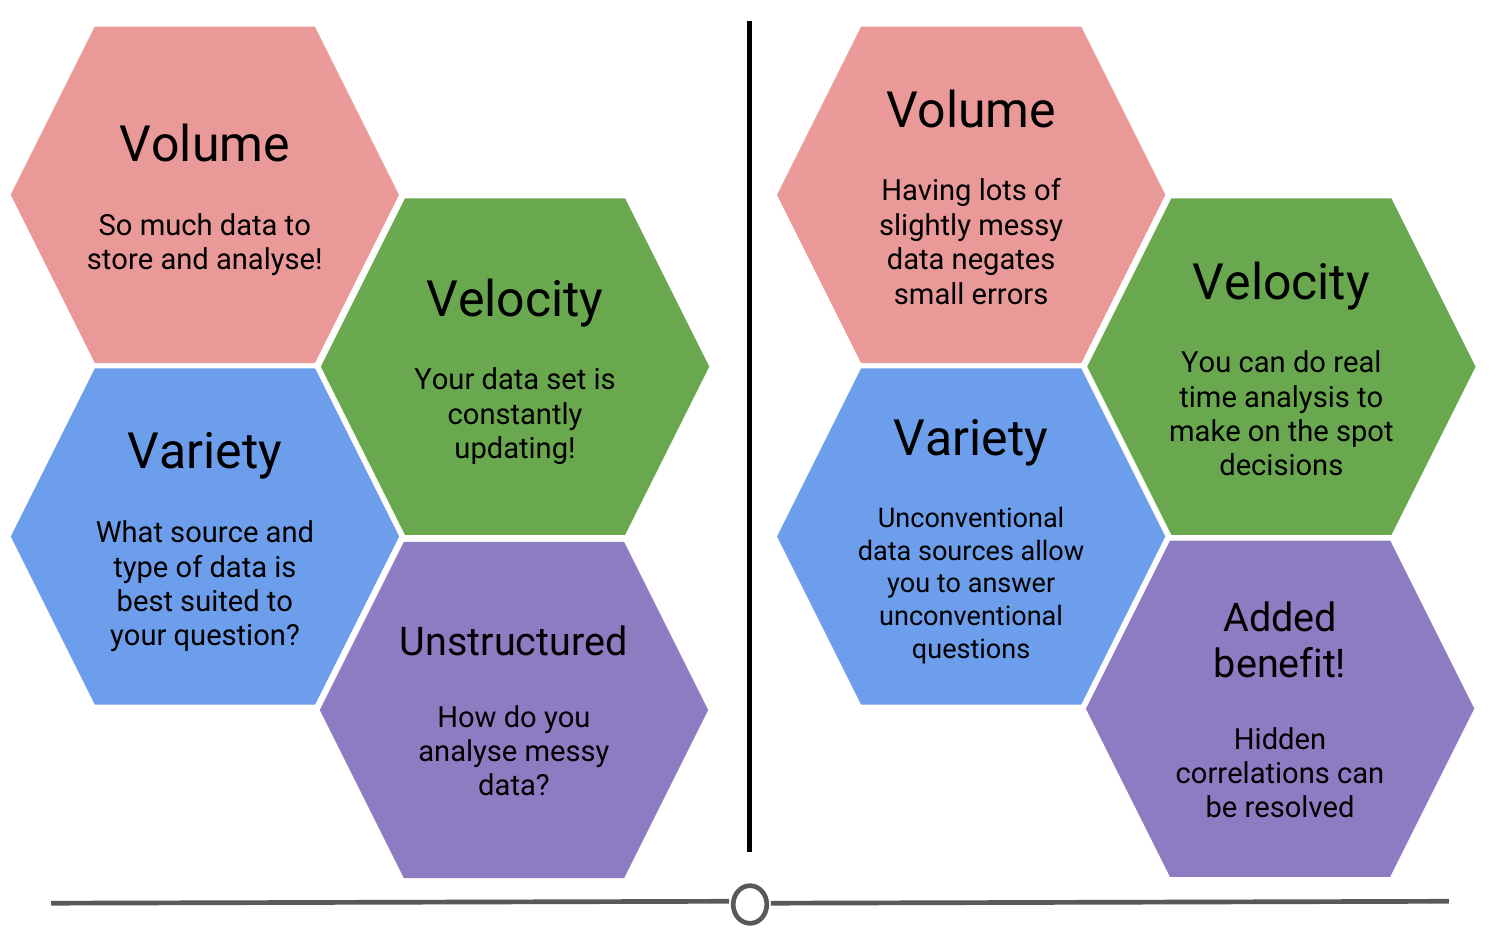
\includegraphics[width=10cm]{big_data.png}
    \caption{Comparing the challenges and benefits to working with big data}
    \label{fig:big_data_pros_cons}
\end{figure}


\chapter{R programming}
Course\cite{course2} outcomes:
\begin{itemize}
    \item how to program in R
    \item how to use R for effective data analysis
    \item how to install and configure software necessary for a statistical programming environment and describe generic programming language concepts as they are implemented in a high-level statistical language
    \item programming in R
    \item reading data into R
    \item accessing R packages
    \item writing R functions
    \item debugging, profiling R code
    \item organizing and commenting R code
\end{itemize}

\section{References}
\begin{itemize}
    \item \url{https://www.rstudio.com/resources/cheatsheets/}
    \item \url{https://iqss.github.io/dss-workshops/R/Rintro/base-r-cheat-sheet.pdf}
    \item \url{https://www.codecademy.com/learn/learn-r/modules/learn-r-introduction/cheatsheet}
    \item \url{http://datasciencefree.com/basicR.pdf}
\end{itemize}

\section{What is R?}
\begin{itemize}
    \item R is a dialect of S.
    \item S is a language that was developed by John Chambers and others at Bell Labs.
    \item S philosophy - wanted to create an interactive environment where the users did not consciously think of themselves as programming. Then as their needs becomes clearer and their sophistication increases, they should be able to slide gradually into programming, when the language and system aspects become more important.
    \item R was created in New Zealand by Ross Ihaka and Robert Gentleman.
    \item syntax is very similar to S.
\end{itemize}

\section{R data types}
\begin{itemize}
    \item "<-" is the assignment operator
    \item "\#" indicates comment
    \item 1:20 creates a sequence 1 to 20
    \item everything in R is an object\\ five basic/atomic classes of objects:
          \begin{itemize}
              \item character
              \item numeric (real numbers)
              \item integer
              \item complex
              \item logical (true/false)
          \end{itemize}
    \item most basic object is a vector
          \begin{itemize}
              \item a vector can only contain objects of the same class
              \item exception - list (represented as a vector) can contain objects of different classes
              \item empty vectors can be created with \texttt{vector()} function
              \item the function has two arguments - class type and length
          \end{itemize}
    \item numbers in R
          \begin{itemize}
              \item numbers are generally treated as numeric objects (i.e. double precision real numbers)
              \item specify \texttt{L} suffix if integer type required
              \item \texttt{Inf} represents infinity
              \item \texttt{NaN} represents an undefined value ("not a number") (e.g. 0/0 or a missing value)
          \end{itemize}
    \item R objects can have the following attributes (\texttt{attributes()} allows you to access the attributes of an object)
          \begin{itemize}
              \item names, dimnames
              \item dimensions (matrices, arrays)
              \item class
              \item length
              \item other user-defined attributes/metadata
          \end{itemize}
    \item creating vectors
          \begin{itemize}
              \item the function \texttt{c()} can be used to create vectors of objects
                    \\ e.g. \texttt{x <- c(0.5, 0.6)} gives a numeric vector of length two with first element as 0.5 and second element as 0.6
              \item example using the function \texttt{vector()} -- \texttt{x <- vector("numeric", length = 10)} -- creates a numeric type vector of length 10 with all values initialized to 0
          \end{itemize}
    \item when different objects are mixed in a vector, \textit{coercion} occurs so that every element in the vector is of the same class
    \item explicit coercion can be done using the \texttt{as.*} functions (e.g. \texttt{as.numeric(vector\_name)} etc.)
    \item when coercion fails, you get \texttt{NA} values as a result
    \item lists
          \begin{itemize}
              \item creating using \texttt{list()} function
              \item example: \texttt{x <- list(1, "a", TRUE, 1+4i)} -- creates a list of number, character, logical and complex
          \end{itemize}
    \item matrices
          \begin{itemize}
              \item matrices are vectors with a dimension attribute
              \item matrix is not a class of objects
              \item the dimension attribute is itself an integer vector of length 2 (nrow, ncol)
              \item example: \texttt{m <- matrix(nrow = 2, ncol = 3)}
              \item \texttt{dim(m)} gives the dimension of the matrix
              \item the matrices are constructed in a column-wise manner
              \item cbind-ing and rbind-ing - column binding and row binding respectively
          \end{itemize}
    \item factors
          \begin{itemize}
              \item used to represent categorical data
              \item can be ordered or unordered
              \item a factor can be thought of as an integer vector where each integer has a label
              \item treated specially by modeling functions like \texttt{lm()} and \texttt{glm()}
              \item function - \texttt{factor()}
              \item also has level
              \item \texttt{unclass(x)} strips the levels and gives integer
              \item the order of the levels can be set using the \texttt{levels} argument to \texttt{factor()}. this is important because the first level is used using the baseline level (which is determined in an alphabetical order by default)
          \end{itemize}
    \item missing values
          \begin{itemize}
              \item missing values are denoted by \texttt{NA} or \texttt{NaN} (\texttt{NaN} is used for undefined mathematical operations)
              \item \texttt{is.na()} is used to test objects if they are \texttt{NA}
              \item \texttt{is.nan()} is used to test objects if they are \texttt{NaN}
              \item \texttt{is.na()} is used to test objects if they are \texttt{NA}
              \item \texttt{NA} can have class - integer, character etc.
              \item A \texttt{NaN} is also a \texttt{NA} but the converse is not true
          \end{itemize}
    \item data frames
          \begin{itemize}
              \item used to store tabular data
              \item represented as a special type of list where every element of the list has to have the same length
              \item each element of the list can be thought of as a column and the length of each element of the list is the number of rows
              \item can store different classes
              \item also have a special attribute called \texttt{row.names}
              \item usually created by calling \texttt{read.table()} or \texttt{read.csv()} or \texttt{data.frame()}
              \item can be converted to a matrix by calling \texttt{data.matrix()}
              \item example: \texttt{x <- data.frame(foo = 1:4, bar = c(T, T, F, F))} creates a data frame of the following kind
                    \begin{table}[H]
                        \begin{tabular}{c c c c c c c c c}
                             &  &  &  &  &  &   & \texttt{foo} & \texttt{bar}   \\
                             &  &  &  &  &  & 1 & 1            & \texttt{TRUE}  \\
                             &  &  &  &  &  & 2 & 2            & \texttt{TRUE}  \\
                             &  &  &  &  &  & 3 & 3            & \texttt{FALSE} \\
                             &  &  &  &  &  & 4 & 4            & \texttt{FALSE}
                        \end{tabular}
                    \end{table}
          \end{itemize}
    \item names attribute
          \begin{itemize}
              \item R objects can also have names, which is very useful for writing readable code and self-describing objects
              \item set using function \texttt{names()}
              \item example: \texttt{names(x) <- c("foo", "bar", "norf")}
              \item list can also have names
              \item matrices have dimnames
          \end{itemize}
\end{itemize}

\section{Dealing with data}
\begin{itemize}
    \item reading data
          \begin{itemize}
              \item \texttt{read.table, read.csv} for reading tabular data
              \item \texttt{readLines} for reading lines of a text file
              \item \texttt{source} for reading R code files (\texttt{inverse of dump})
              \item \texttt{dget} for reading in R code files (\texttt{inverse of dout})
              \item \texttt{load} for reading in saved workspaces
              \item \texttt{unserialize} for reading single R objects in binary form
          \end{itemize}
    \item writing data
          \begin{itemize}
              \item \texttt{write.table}
              \item \texttt{writeLines}
              \item \texttt{dump}
              \item \texttt{dput}
              \item \texttt{save}
              \item \texttt{serialize }
          \end{itemize}
    \item \texttt{read.csv} has comma as separator while \texttt{read.table} has space as separator
    \item reading lager datasets with \texttt{read.table}
          \begin{itemize}
              \item read the help page for \texttt{read.table}
              \item have a rough idea of the amount of data that will be read - to understand if you have enough memory to store the dataset
              \item how to calculate this?
          \end{itemize}
    \item

\end{itemize}

\nocite{elegantbook}
\printbibliography

\end{document}